\documentclass[
 a4paper,
 12pt,
 parskip=half
 ]{scrreprt}
%\setcounter{secnumdepth}{0}
 
\usepackage{settings}

\usepackage{mathpkgs}
\usepackage{mathcmds}

\usepackage[]{fancy_thm}

\usepackage{siunitx}
\sisetup{locale = DE}

\theoremstyle{plain}

\theoremstyle{definition}
%\newtheorem{defn}{Definition}
%\newtheorem{folg}[thm]{Folgerung} 
%\newtheorem{rmrk}[thm]{Bemerkung} 
%\newtheorem{deno}[thm]{Bezeichnungen}
%\newtheorem{exmp}[thm]{Beispiel}
%\newtheorem{aufg}[thm]{Aufgabe} 
%\newtheorem{prgp}[thm]{} % Numbered paragraph

\newtheorem*{rmrk*}{Bemerkung}
%\newtheorem*{exmp*}{Beispiel}
\newtheorem*{defn*}{Definition}
%\newtheorem*{deno*}{Bezeichnungen}

\DeclareMathOperator{\MB}{MB}
\DeclareMathOperator{\BGK}{BGK}

\newcommand{\thr}{\texttt{threshold}}

\hypersetup{
  pdftitle={MOSIM2},
  pdfauthor={Jonas Hippold},
  hidelinks
}

%opening
\title{%
  Vorlesung\\
  MoSim - Modellierung und Simulation 2
}

\subtitle{Sommersemester 2018}

\author{%
  Vorlesung: Jun.-Prof. Dr. Christian Mendl\\
  Mitschrift: Jonas Hippold
}

\begin{document}

\maketitle

\tableofcontents

\chapter{Einleitung}

Folien

\chapter{Grundlagen künstlicher neuronaler Netze}
artificial neural networks (ANN)

Michael Nielsen: \url{neuralnetworksanddeeplearning.com}

\textbf{Motivation:} Handschrifterkennung
\begin{center}
  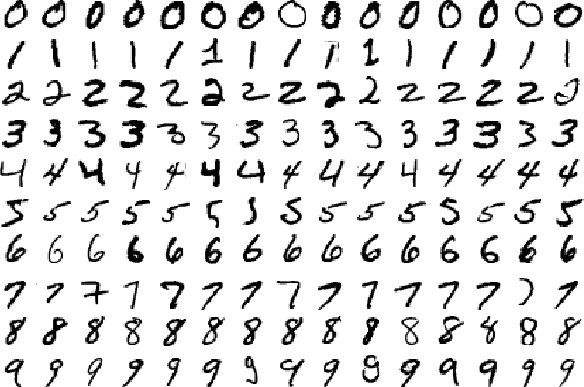
\includegraphics[width=8cm]{img/handwriting.jpg}
\end{center}

\textbf{Ziel:} Beliebige handschriftliche Zeichen automatisch identifizieren.

\textbf{Menschliches Gehirn:} Visueller Kortex, Hierarchie $V_1 \to V_2 \to
\ldots \to V_5$, wobei die Abstraktion mit dem Index steigt. Vergleiche hierzu
D. Hubel, T. Wiesel, Nobelpreis 1981.

Der ``konventioneller'' Programmieransatz (imperatives Programm mit
if-then-else, for-Schleifen, usw.) stellt sich als mühselig bzw. schwierig
umzusetzen heraus.

ANNs: ``Trainieren'' des Netzes mit vielen (zehntausende oder mehr)
Trainingspaaren $(x^{(i)}, y^{(i)})$. $x^{(i)}$ ist ein Bitmap-Bild, $y^{(i)}$
die zugehörige Ziffer.

Referenz: (Benchmark-)Datensatz MNIST (modified NIST\footnote{%
  National Institute for Standards and Technology (USA)
}). Hier ist jedes $x^{(i)}$ ein $28 \times 28$ Bitmap mit Graustufen.

\clearpage

\section{Perzeptrons}
Frank Rosenblatt 1950, 1960er: Vorläufer ``moderner'' ANN.
\begin{center}
  \begin{minipage}{.45\textwidth}
    \begin{center}
      \includegraphics[]{img/single_perceptron}
    \end{center}
  \end{minipage}
  \begin{minipage}{.45\textwidth}
    \[ \texttt{output} =
      \begin{cases}
        0, & \sum_j w_j x_j \le \texttt{threshold}, \\
        1, & \sum_j w_j x_j > \texttt{threshold}.
      \end{cases}
    \]
    $\texttt{output} = 1$ bedeutet, dass die Zelle ``feuert''.
  \end{minipage}
\end{center}

\subsubsection*{Beispiel: Entscheidungsprozess ``Soll ich das Festival
  besuchen?''}

Kriterien:
\begin{enumerate}
\item Wetter
\item Kommen Freunde mit?
\item Gut erreichbar mit öffentlichen Verkehrsmitteln?
\end{enumerate}

$x_1 = 1$ ... Wetter ist gut, $x_1 = 0$ ... Wetter ist schlecht.

Szenario 1: ``Will unbedingt, aber nur falls Wetter in Ordnung.''
\[ w_1 = 6, \quad
  w_2 = 2, \quad
  w_3 = 2, \quad
  \thr = 5. \]
Die Entscheidung hängt nur vom Wetter ab.

Szenario 2:
\[ w_1 = 6, \quad
  w_2 = 2, \quad
  w_3 = 2, \quad
  \thr = 3. \]
Besuche das Festival, falls das Wetter gut ist, oder wenn 2. und 3. gleichzeitig
erfüllt werden.

\subsubsection*{Perzeptron-Netzwerk}
\begin{center}
  \includegraphics[]{img/ann}
\end{center}
Jede Zelle hat eigene Gewichte und Thresholds.

Der Output einer Zelle im ersten Layer wird an mehrere Zellen des zweiten Layers
weitergeleitet. Jede Zelle produziert aber nur einen Output-Wert, der mehrfach
kopiert wird. 

Kompakte Notation: Bias $b := - \thr$
\[ \texttt{output} =
  \begin{cases}
    0, & \sum_j w \cdot x + b \le 0, \\
    1, & \sum_j w \cdot x + b < 0
  \end{cases}
\]
mit den Gewichts- bzw. Eingabevektoren $w = (w_1, w_2, \ldots)^\top$ und $x =
(x_1, x_2, \ldots)^\top$.

\subsubsection*{Abbildung eines NAND-Gatters als Perzeptron}
\[ w_1 = -2, \quad w_2 = -2, \quad b = 3 \]
\begin{center}
  \begin{minipage}{6cm}
    \begin{center}
      \begin{tabular}{cc|c}
        $x_1$ & $x_2$ & \texttt{output} \\
        \hline
        0 & 0 & 1 \\
        0 & 1 & 1 \\
        1 & 0 & 1 \\
        1 & 1 & 0
      \end{tabular}
    \end{center}
  \end{minipage}
  \begin{minipage}{6cm}
    Notation in der Elektrotechnik für NAND-Gatter:
    \begin{center}
      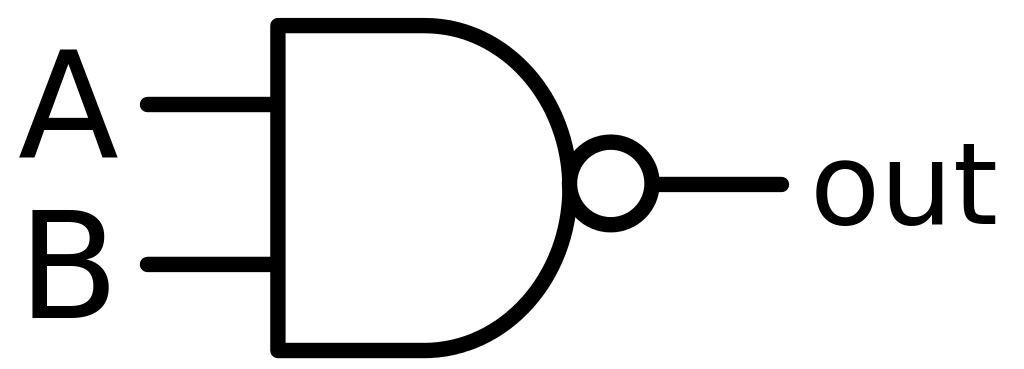
\includegraphics[width=3cm]{img/nand}
    \end{center}
  \end{minipage}
\end{center}

Das NAND-Gate ist universell, man kann beliebige digitale Schaltungen aus
Verbindungen dieser Gatter zusammen stellen. Beispiel:
\begin{align*}
  \texttt{NOT} \, x
  &= x \, \texttt{NAND} \, x, \\
  x_1 \, \texttt{OR} \, x_2
  &= (\texttt{NOT} \, x_1) \, \texttt{NAND} \, (\texttt{NOT} \, x_2) \\
\end{align*}
Idee bei ANN: Optimiere die Gewichte und Bias-Werte beim ``Training'', um die
gewünschte Ausgabe zu erhalten. Damit ``lernt'' das Netzwerk, die geforderte
Ausgabe zu erzeugen.

\section{Neuronen mit Sigmoid-Aktivierungsfunktion}
Eine Schwierigkeit des Perzeptron-Modells im Hinblick auf die Optimierung der
Parameter ist, dass die Ausgabe keine stetige Funktion ist. Damit ist sie
insbesondere nicht differenzierbar und man kann keinen Gradienten definieren.

Als Abhilfe ersetzt man die binäre Ausgabefunktion durch eine stetige Funktion
$\sigma(w \cdot x + b)$, die \emph{Sigmoid-Aktivierungsfunktion}, zum Beispiel
\[ \sigma(z) = \rez{1+e^{-z}}. \]
\begin{center}
  \includegraphics[scale=.85]{img/sigmoid}
\end{center}

Es gilt $\lim_{z \to -\infty} \sigma(z) = 0$ und $\lim_{z \to \infty} \sigma(z)
= 1$.

Die genaue Form von $\sigma(z)$ ist nicht entscheidend, wichtig ist die
Differenzierbarkeit. Auch andere Aktivierungsfunktionen sind gebräuchlich.

\section{Die Topologie künstlicher Feedforward-Netze}
\subsubsection*{Feedforward-Netzwerk}
Information ``fließt'' stets von ``links nach rechts'', das heißt es handelt
sich um einen azyklischen gerichteten Graph, es gibt keine ``Feedback-Loops''.

Input Layer: Zum Beispiel einzelne Pixelwerte eines Bildes bei Schrifterkennung.
MNIST: $28 \times 28$ Pixel, also $28^2 = 784$ Input-Einheiten.

``Deep'' network: Es gibt mehrere Zwischenschichten. Feedforward-Netze
unterscheiden sich somit von ``Recurrent Neural Networks'' (Rekurrente Netze)
mit Feedback-Loops.

\begin{center}
  \includegraphics[scale=.85]{img/ann_deep}
\end{center}

\section{Ein einfaches Netzwerk zur Klassifizierung handschriftlicher Ziffern}
Zwei Teilprobleme:
\begin{itemize}
\item Segmentierung: Einteilung eines Bildes von Handschrift in einzelne Zeichen
\item Eigentliche Klassifizierung: Zuordnung der Ziffern zu den segmentierten
  Bildern.
\end{itemize}
Hier behandeln wir die eigentliche Klassifizierung.

\subsubsection*{Netzwerk-Topologie}
\begin{center}
  \includegraphics{img/ann_handwriting}
\end{center}
Ziffer mit höchster ``Aktivität'' (größter Ausgabewert des entsprechenden
Neurons) wird als Klassifizierungswert des Netzwerks interpretiert.

\subsubsection*{Heuristische Interpretation}
Nervenzellen im ``Hidden Layer'' erkenn charakteristische Segmente von Ziffern,
zum Beispiel:
\[ \begin{matrix}
    \square & \square & \square & \square & \square & \square & \square \\
    \square & \blacksquare & \blacksquare & \blacksquare &
    \blacksquare & \blacksquare & \square \\
    \square & \square & \square & \square & \square & \square & \square \\
    \square & \square & \square & \square & \square & \square & \square \\
    \square & \square & \square & \square & \square & \square & \square \\
    \square & \square & \square & \square & \square & \square & \square \\
    \square & \square & \square & \square & \square & \square & \square \\
  \end{matrix}
\]
Diese Eingabe könnte zu einer 5 oder 7 gehören.

\section{Lernen mittels Gradientenverfahren}
\subsubsection*{Trainieren und Testen}
Training: MNIST-Datensatz enthält 60000 handschriftliche
Ziffern als Bilder ($28 \times 28$ Grauwerte) und entsprechende Klassifizierung
von 250 Personen.

Test: 10000 weitere handschriftliche Ziffern einer \emph{anderen} Gruppe von
250 Personen.

Eingabe: $x \in [0,1]^{784}$ (Vektor aus Grauwerten)

Klassifizierung: $y(x) \in \{0,1\}^{10}$ (Indikatorfunktion), Beispiel:
\[ y(x) = (0,0,0,0,0,0,1,0,0,0,0) \simeq 6. \]

(Quadratische) Kostenfunktion (``cost'' bzw. ``loss funciton'')
\[ C(w,b) = \rez{2n} \sum_{j=1}^n \| y(x^{(i)}) - a(x^{(i)}, w, b) \|^2. \]
$w, b$ ist die Menge aller Gewichte und Bias-Werte des Netzwerks, jede Zelle hat
individuelle Parameter.

$a(x,w,b)$: Ausgabe des Netzwerks für Eingabe $x$.

Ziel: Das Netzwerk klassifiziert Ziffern korrekt, also
\[ C( w, b ) \approx 0. \]

\begin{rmrk*}
  Die Kostenfunktion ist eine glatte Funktion der Netzwerk-Ausgabe (im Gegensatz
  zur \emph{Anzahl} der korrekt klassifizierten Bilder).
\end{rmrk*}

Fasse Netzwerk-Parameter als $v = (w,b)$ zusammen.

\subsubsection*{Gradientenverfahren}
Wiederholtes Anwenden von
\[ v \to v' = v - \eta \nabla C \]
mit der ``Lernrate'' $\eta$, $\nabla C$ ist der Gradient bezüglich $v$.

Schwierigkeit hierbei:
\[ C = \rez{n} \sum_{j=1}^n C_{x^{(j)}} \]
mit 
\[  C_x = \rez{2} \| y(x) - a(x,w,b) \|^2 \]
und damit
\[ \nabla C = \rez{n} \sum_{j=1}^n \nabla C_{x^{(j)}}. \]
Das ist eine Summe über alle Trainingspaare $(x^{(i)},y^{(i)})$, die Auswertung
ist ``teuer'' (großer Rechenaufwand), zum Beispiel 60000 Summanden bei
MNIST.

\subsubsection*{Ausweg}
Approximiere den Gradienten mittels kleiner, zufällig ausgewählter Teilmenge
aller Trainingspaare (sogenannter ``mini batch'')
\[ \{ (x(j_1), y(j_1)), \ldots, (x(j_m), y(j_m)) \}. \]
Dann ist
\[ \nabla C \approx \rez{m} \sum_{i=1}^m \nabla C_{x(j_i)} \]
für einen Schritt des Gradientenverfahrens (mit neuem, disjunkten mini batch für
den nächsten Schritt).

Explizit mit $w_k$ und $b_l$ als Gewichte und Bias-Werte:
\begin{align*}
  w_k &\to w'_k = w_k - \eta \rez{m} \sum{i=1}^m \pdiff{C_{x(j_i)}}{w_k} \\
  b_l &\to b'_k = b_k - \eta \rez{m} \sum{i=1}^m \pdiff{C_{x(j_i)}}{b_l}
\end{align*}

\begin{rmrk*}
  Ein Grenzfall ist $m=1$, das sogenannte ``online learning''. Die
  Netzwerk-Parameter werden basierend auf einem einzelnen Trainingspaar
  aktualisiert.

  Dieses Verfahren setzt man zum Beispiel bei der Echtzeit-Generierung der Daten
  ein, dann ist keine Speicherung der Trainingspaare notwendig.

  Aber: Große Schwankungen in der Gradientenrichtung sind möglich.
\end{rmrk*}

Verbesserte Alternativen zum ``stochastic gradient descent'' sind ebenfalls
gebräuchlich, zum Beispiel Adam optimizer.

\section{Der Backpropagation-Algorithmus}
Ziel: Effiziente Berechnung des Gradienten der Kostenfunktion $\lambda C$
bezüglich $v = (w,b)$.
\[ C(v) = \sum_{j=1}^n C_{x^{(j)}}(v), \]
somit
\[ \nabla C =  \sum_{j=1}^n \nabla C_{x^{(j)}} (v). \]

Hier: Einzelner Inputvektor $x$.

Betrachte ein Netzwerk mit $L$ Schichten. $a_j^l$ bezeichne die Ausgabe des
$j$-ten Neurons in Schicht $l$.
\[ a_j^l = \sigma \left( \sum_k w_{jk}^j a_k^{l-1} + b_j^l \right) \]
Matrix-Vektor-Notation:
\[ a^l = \sigma( \underbrace{w^l \cdot a^{l-1} + b^l}_{=: z^l}), \]
wobei hier $\sigma$ komponentenweise angewendet wird.

Hilfsgröße: $\delta_j^l := \pdiff{C}{z_j^l}$, dann gilt mit der Kettenregel (K)
\[ \delta_j^L = \pdiff{C}{z_j^L} \overset{\text{(K)}}{=}
  \sum_k \pdiff{C}{a_k^L} \pdiff{a_k^L}{z_j^l} =
  \pdiff{C}{a_j^L} \cdot \sigma'(z_j^L), \]
weil $\pdiff{a_k^L}{z_j^l} = 0 $ für $k \ne j$ und $a_k^L = \sigma(z_k^L)$.

Zum Beispiel für $C = \rez{2} \| a^L - y \|^2 $:
\[ \pdiff{C}{a_j^L} = a_j^L - y_j. \]

Matrix-Vektor-Notation:
\[ \delta^L = \diag( \sigma'(z^L)) \cdot \nabla_{a^L} C. \tag{BP1} \]
Ähnliche Berechnung (siehe Tutor-Aufgabe):
\[ \delta^l = \diag( \sigma'(z^l)) \cdot (w^{l+1})^\top \cdot \delta^{l+1}
  \tag{BP2} \]
für alle $l < L$, wobei das erste $\cdot$ eine Matrix-Matrix-Multiplikation
darstellt.

Die Bezeichnung Backpropagation kommt von dieser Berechnungsvorschrift. Der
Gradient ``propagiert rückwarts'' von Schicht $l+1$ zu Schicht $l$.

Mit analoger Berechnung erhält man für die Bias-Werte
\[ \pdiff{C}{b_j^l} = \delta_j^l \tag{BP3} \]
und für die einzelnen Gewichte
\[ \pdiff{C}{w_{jk}^l} = a_k^{l-1} \delta_j^l. \tag{BP4} \]

Insbesondere: Der Gradient ist klein für $\sigma'(z_j^l) \approx 0$, das heißt
falls die Nervenzelle saturiert ist. Für $|z| \gg 0$ tritt also keine große
Veränderung der Gewichte auf. Das kann auch hinderlich sein und das Lernen der
Zelle verlangsamen.

\begin{rmrk*}
  Wiederholtes Anwenden von (BP2) führt auf
  \[ \delta^l = \diag( \sigma'(z^l)) \cdot (w^{l+1})^\top \cdot
    \diag(\sigma'(z^{l+1})) \cdot (w^{l+2})^\top \cdot \ldots \cdot \diag(\sigma'(z^L))
    \cdot \nabla_{a^L} C. \]
\end{rmrk*}

\subsubsection*{Algorithmus}
Direkte Implementierung von (BP1) bis (BP4)

Gegeben: Input-Vektor $x$
\begin{enumerate}
\item Feedforward Pass (Durchlauf): \\
  for each $l = 1, 2, \ldots, L$:
  \begin{align*}
    z^l &= w^l a^{l-1} + b^l \qquad (\text{with } a^0 = x) \\
    a^l &= \sigma(z^l)
  \end{align*}
\item Berechne BP1:
  \[ \delta^L = \diag(\sigma'(z^L)) \cdot \nabla_{a^L} C \]
\item Backpropagate, BP2: \\
  for each $l = L-1, L-2, \ldots, 1$:
  \[ \delta^l = \diag( \sigma'(z^l)) \cdot (w^{l+1})^\top \cdot \delta^{l+1} \]
\item Berechne Gradienten, BP3, BP4:
  \[ \pdiff{C}{w_{jk}^l} = a_k^{l-1} \delta_j^l, \qquad
    \pdiff{C}{b} = \delta_j^l. \]
\end{enumerate}

\begin{rmrk*}
  \begin{itemize}
  \item Der Algorithmus wäre auch für ``individuelle'' Aktivierungsfunktionen
    (für jedes Neuron eigene Funktion $\sigma_j^l$) anwendbar.
  \item In der Praxis steigert man die Effizienz durch eine Matrix-Formulierung
    für einen mini-batch. Das heißt, anstatt den Algorithmus nacheinander auf
    $x^{(j_1)}, x^{(j_2)}, \ldots, x^{(j_m)}$ anzuwenden, speichert an die
    auftretenden Vektoren als Spalten einer Matrix:
    \[ ( z^{l^{(j_1)}} | z^{l^{(j_2)}} | \cdots | z^{l^{(j_m)}}), \quad
      ( a^{l^{(j_1)}} | a^{l^{(j_2)}} | \cdots | a^{l^{(j_n)}}), \quad
      ( \delta^{l^{(j_1)}} | \delta^{l^{(j_2)}} | \cdots |
      \delta^{l^{(j_n)}}). \]
    Hintergrund ist die optimale Verwendung des Caches bei der Berechnung mit
    dem Computer. Eine Matrix-Matrix-Multiplikation ist schneller als $n$-mal
    eine Matrix-Vektor-Multiplikation auszuführen.
  \item Naiver Ansatz: Die Numerische Approximation des Gradienten durch 
    Differenzenquotienten, das heißt
    \[ \pdiff{C}{v_j} \approx \frac{C(v+h e_j) - C(v)}{h} \]
    mit $0 < h \ll 1$, ist in der Praxis zu rechenaufwendig. Man müsste die
    Kostenfunktion für jeden Eintrag der Gewichtsmatrizen und Bias-Vektoren neu
    auswerten (Feedforward-Pass durch das Netzwerk).

    Der Backpropagation-Algorithmus liefert alle Gradienten mit nur einem
    Feedforward- und Backward-Pass.
  \end{itemize}
\end{rmrk*}

\section{Verbesserungen beim Trainieren künstlicher
  neuronaler Netze}
\subsection{Cross-Entropy Kostenfunktion}
Modellbeispiel: Einzelne Nervenzelle mit Ausgabe
\[ a = \sigma( wx + b ), \qquad w,b \in \real. \]
$x=1$, gewünschte Ausgabe $y=0$.

Training mit dem Gradientenverfahren angewendet auf $w$, $b$ mit Kostenfunktion
\[ C= \rez{2} (y-a)^2. \]

Szenario 1: Startwerte $w = \num{.6}$, $b = \num{.9}$. Anfänglich ist also
\[ a = \num{.817}. \]

Lernrate $\eta = \num{.15}$. Nach 300 Iterationen ist
\[ w = \num{-1.28}, \qquad b = \num{-.98}, \qquad a = \sigma(wx + b) =
  \num{.09}. \]

Szenario 2: Startwerte $w = 4$, $b = 4$. Anfänglich ist also
\[ a = \num{.817} \]

Lernrate $\eta = \num{.15}$.

\begin{center}
  \includegraphics{img/grad_descent}
\end{center}

Wunsch: Die Nervenzelle sollte in Szenario 2 schneller lernen, da die Abweichung
von $y$ größer ist als in Szenario 1. Aber das Gegenteil ist der Fall.
\end{document} 